\section{Results}
\label{section:dsr_results}

\subsection{Really Simple Drools}

The Really Simple Drools Language (RSD) acted as a training ground for our new projections.

\subsubsection{Context-Aware Colour Scheme}
After the default text projection, the first projection we made was giving the text a colour scheme.
This form or augmentation in IDEs is probably the most basic that we see.
Available in structured editors since the 1980s\cite{cowlishaw1987lexx}, syntax highlighting displays text in various colours and fonts according to the meaning of the terms.
Syntax highlighting is helpful for the comprehension of code, as least for small code bases\cite{sarkar2015impact}.

Developers at our host organisation use Eclipse or IntelliJ Community Editions to edit code, neither of which has syntax highlighting for Drools. Thus, the addition of this feature would immediately benefit them.
However, IntelliJ IDEA, the paid version, already provides this feature for Drools.
We extended the colour scheme to indicate whether the selection is looking for a positive or negative match to offer another visual augmentation that we considered valuable.
Figure \ref{fig:colorscheme} shows this projection.

\begin{figure}[h]
    \centering
    \fbox{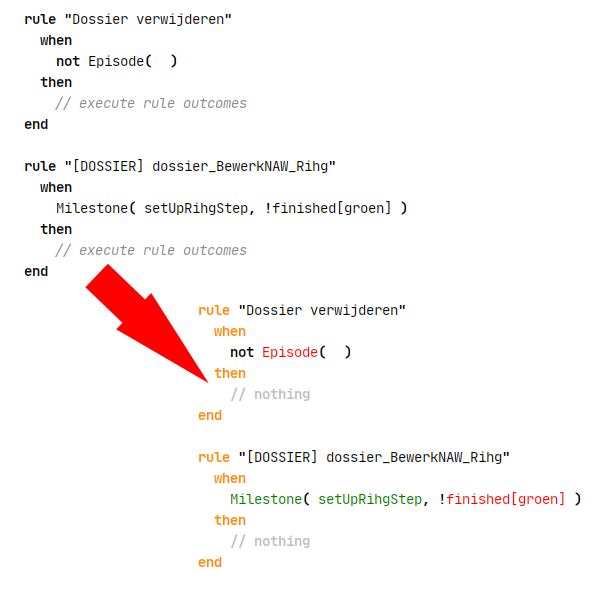
\includegraphics[width=0.66\textwidth]{Sections/images/coloredTextProjection_P.png}}
    \caption{Context aware colour scheme}
    \label{fig:colorscheme}
\end{figure}

\texttt{FactDeclaration} references contained by \texttt{NotCondition} nodes and \texttt{FactProperty} references that are part of a \texttt{NotPredicate} node appear highlighted in Red.
\texttt{ExistCondition} and \texttt{IsPredicate} nodes have their content coloured green.
We did not test whether this improved understanding.

\subsubsection{Summary Projection}

Our next projection allows developers to have a quick overview of the \texttt{Rule} nodes and the complexity of those nodes.
Figure \ref{fig:summaryProjection} shows that the developers can get an overview of both the number of \texttt{Rule} nodes and the number of \texttt{FactDeclaration} references in each of the \texttt{Rule} nodes.

\begin{figure}
    \centering
    \fbox{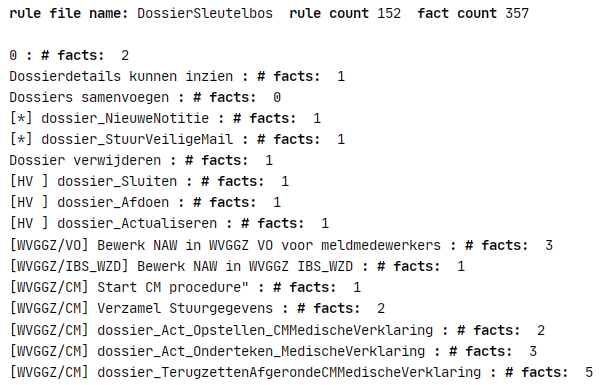
\includegraphics[width=0.66\textwidth]{Sections/images/summaryProjection_P.png}}
    \caption{Summary projection}
    \label{fig:summaryProjection}
\end{figure}

The building of this projection only required adjusting two editors.
The \texttt{Rule} node count and \texttt{FactDeclaration} reference count were added to the \texttt{File} Concept editor using Read-Only Model Access to count the descendants of the \texttt{File} node that are \texttt{Rule} nodes and \texttt{FactDeclaration} references.
The \texttt{Rule} Concept editor was adjusted only to show the \texttt{Rule} nodes title and, again using the model access, the count of the descendants of the \texttt{Rule} that were \texttt{FactDeclaration} references.

Whilst this may look like a report that any language workbench could create, the \texttt{File} node name and the names of the \texttt{Rule} nodes are editable in this projection.

\subsubsection{Filtering}
Whilst investigating how to handle extensive collections of rules, we looked to domains that already handle extensive collections of items.
The domain of data analysis has a long history of handling large volumes.
Among their two most used tools for exploration are sorting and filtering.

The nature of business rules lends them to some projectional options that would not make sense with other programming styles.
Because of the independent nature of the rules, filtering lends itself to the business rules style.
The semantic meaning of the order of business rules means we did not find a good use case for sorting rules.
So, we decided to implement a filtering projection.

Whilst filtering occurs in other places in the coding pipeline, such as deciding on what code completion to present\cite{hou2010towards} and version control visualisation\cite{yoon2013visualization}, we were unable to find any research on applying filtering directly to code files.
Consequently, we think what we present here is an original idea.

\texttt{Rule} nodes that use the same \texttt{FactDeclaration} references or \texttt{FactProperty} references are likely to be related.
Thus, these seemed the obvious items to filter.
We created a projection where if the developer filtered by a \texttt{FactDeclaration} or a \texttt{FactProperty}, the projection would filter out all \texttt{Rule} nodes that did not contain references to the nodes.
Once the \texttt{Rule} nodes were filtered, the projection only shows \texttt{FactDeclaration} nodes and \texttt{FactProperty} nodes that are referenced by those \texttt{Rule} nodes.

In our implementation, shown in figure \ref{fig:filteringProjection} on the following page, we show three places where we use intentions to filter the code.
The first is an intention associated with a \texttt{FactDeclaration} node.
We show the outcome of choosing this filter on the righthand side of figure \ref{fig:filteringProjection}.
The second intention is on a \texttt{FactProperty} node.
As the \texttt{FactProperty} node is a child of a \texttt{FactDeclaration} node, we see both intentions.
The third highlighted intention is on a \texttt{FactProperty} reference.
It also shows an intention associated with a \texttt{FactDeclaration} reference in the \texttt{FactSelector} node that holds the \texttt{FactPropertyReference} as a child.

\begin{sidewaysfigure}
    \centering
    \fbox{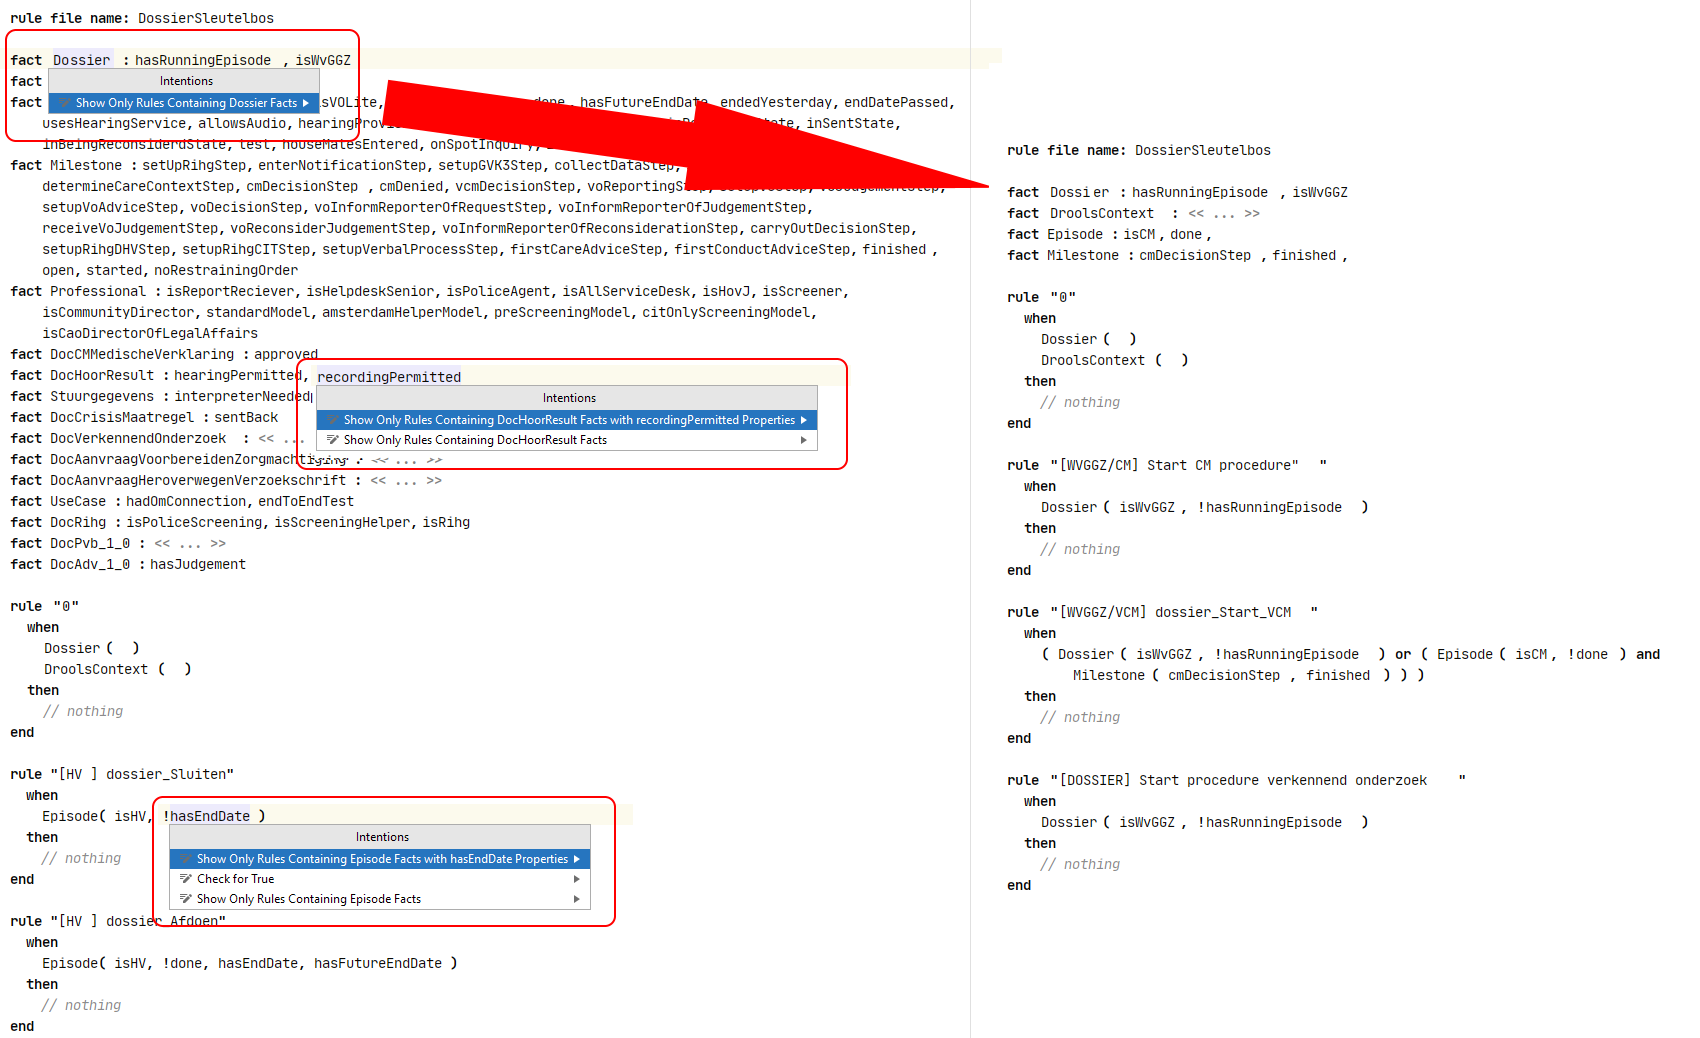
\includegraphics[width=0.99\textwidth]{Sections/images/filteringProjection.png}}
    \caption{Filtering projection}
    \label{fig:filteringProjection}
\end{sidewaysfigure}

One of our guidelines was, as much as possible, to build our projections as separate languages, non-invasively extending RSD.
In our first approach at the filtering, we failed on this count by invasively adding properties to the \texttt{FactDeclaration} and \texttt{FactProperty} Concepts of the RSD to determine whether they were visible.

Our following approach created subclasses of the \texttt{FactDeclaration}, \texttt{FactProperty} and \texttt{File} Concepts.
This approach, however, requires running a macro on the code file to migrate \texttt{FactDeclaration}, \texttt{FactProperty} and \texttt{Files} nodes to \texttt{FilteredFact}, \texttt{FilteredFactProperty}, and \texttt{FilteredFile} nodes.
This migration means that the \texttt{FilteredFile} could now only be used by languages that extend our new filtered language.

Our final approach was to add a \texttt{Filter} Concept, reference the filtered nodes, and have the editors make the visibility calculations based on this singleton node.
Whilst more complex, this removed the need for invasive changes and allowed other languages to combine with the filtering language.

Filtering is a handy projection.
However, it breaks Dijkstra's rule ``the purpose of abstraction is not to be vague but to create a new semantic level in which one can be absolutely precise.''\cite{dijkstra1972humble}.
This projection fails this rule by hiding some of the meaning of the code.
This projection has no way of containing the whole code whilst a filter is applied.
However, we feel that so long as there is a clear indication that a filter is applied, then we see this as a tool in a similar vein to the code collapsing functionality found in most modern-day editors.

\subsubsection{Table}
Thus far, our projections have been textual ones that other non-projectional language workbenches could implement.
Creating a table was our first non-parsable projection.

We choose the table projection based on the observations of Miller\cite{miller1956magical} about the number of items people can retain in their memory.
This observation leads us to conclude that the fewer essential items that are off the screen and, therefore, in the developers' memory, the better.

Figure \ref{fig:tableProjection1} on page \pageref{fig:tableProjection1} shows our rudimentary first table.
This simple table has only the ``name'' property and the ``when'' children of the \texttt{Rule} nodes in the \texttt{File} node.
We implemented this projection using the tables extension in the MPS-Extension plug-in, created by Sascha Lißon.

\begin{sidewaysfigure}
    \centering
    \fbox{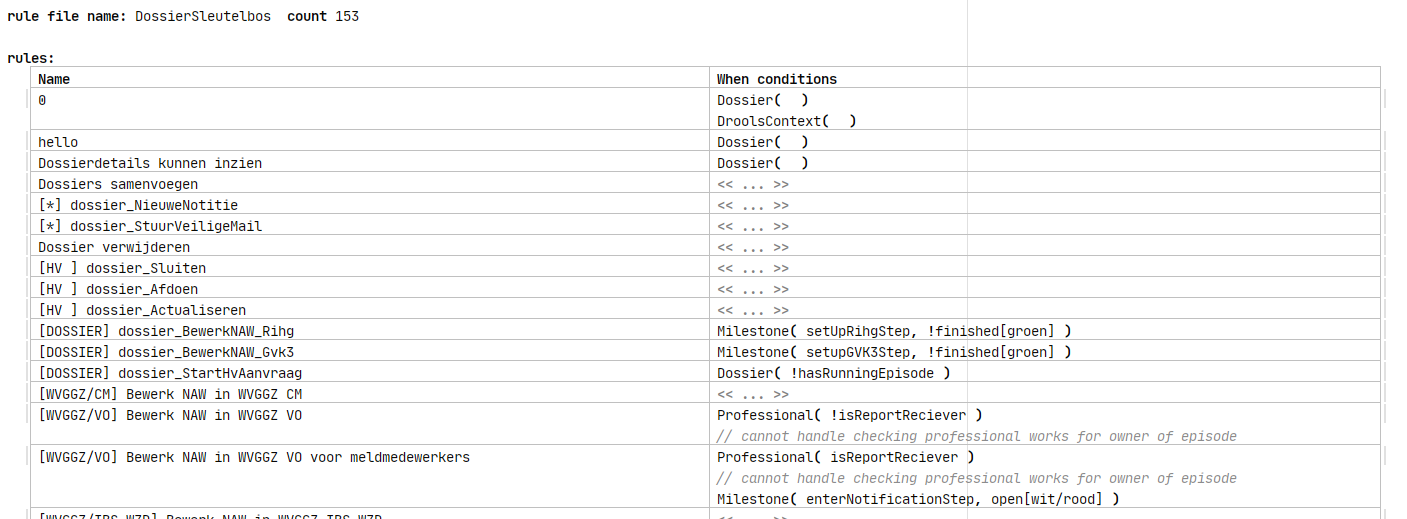
\includegraphics[width=0.99\textwidth]{Sections/images/tableProjection1.png}}
    \caption{Table projection}
    \label{fig:tableProjection1}
\end{sidewaysfigure}

\subsubsection{Crosstab}
Our next tabular projection is a crosstab inspired by a decision table.
Figure \ref{fig:crosstabProjection1}, on page \pageref{fig:crosstabProjection1}, shows our implementation of the crosstab.
Because of the large amount of screen real estate that this projection uses, we only present a truncated view of the table.

The reason behind this projection is that the previous table does not give any visual cues as to how \texttt{Rule} nodes are related.
With a crosstab, one can easily see which rules contain the same facts.

The rows of the crosstab represent the rules, with the name in the left-most column.
The columns represent the facts.

The cells show the facts used in each rule.
A number preceded by a hash symbol indicates if a rile requires a fact.
The number represents the ordinal order of when the facts appear in the conditions.
Thus, the first occurrence of a fact is represented by ``\#1''.
If there are multiple occurrences of a fact within a rule, multiple numbers will appear in the same cell.

In the figure, a close-up shows that all the details of the selected fact are available in the inspector panel.

At the top, we can see an immediate problem with a crosstab
If we have the whole \texttt{File} node represented, then the table will be very sparse.

\begin{sidewaysfigure}
    \centering
    \fbox{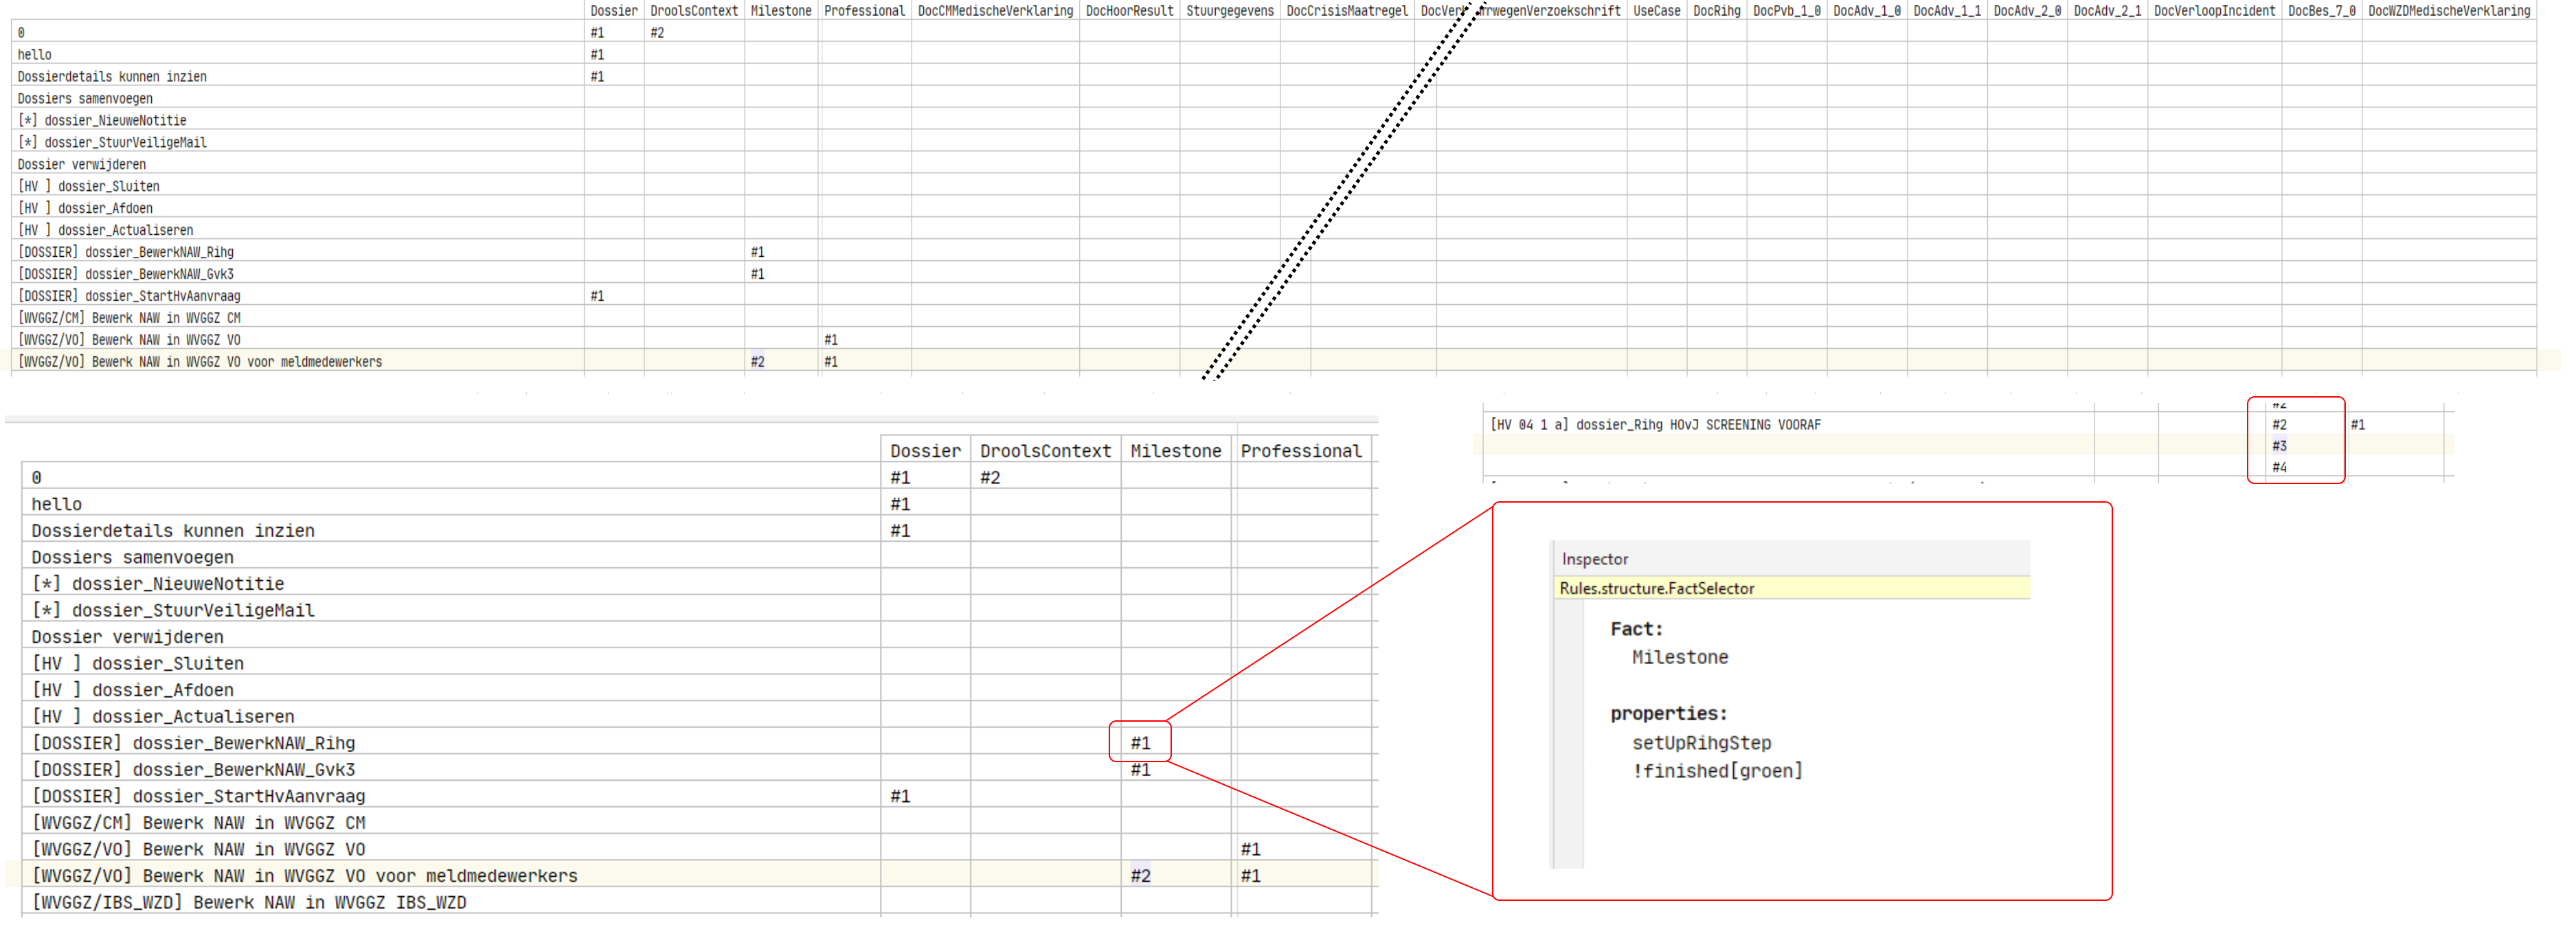
\includegraphics[width=0.99\textwidth]{Sections/images/crosstabProjection1.png}}
    \caption{Crosstab projection}
    \label{fig:crosstabProjection1}
\end{sidewaysfigure}

Everything is editable in this table, including deleting a \texttt{FactDeclarationSmartRef} from a \texttt{Rule} node.
The table plug-in and MPS enabled most of the editing in the projection by default.
An extra editing feature we added to this table was the ability to delete a \texttt{FactDeclaration} node and all the related references from all the \texttt{Rule} nodes in the \texttt{File} node by deleting a fact column.
The code shown in figure \ref{fig:tableFactDeletion}, on page \pageref{fig:tableFactDeletion}, shows how we can walk the trees in each \texttt{Rule} to delete unary conditions and convert the non-deleted side of binary conditions into unary conditions to allow this \texttt{FactDeclaration} reference deletion.

From the ``on delete'' section of the vertical section, we loop through all the \texttt{Rule} nodes to remove the references and rearrange the conditions in the AST.
This projection calls a recursive ``pruneCondition'' method to walk the tree to detach \texttt{FactSelector} nodes containing references to the \texttt{FactDeclaration}.
If it is a unary \texttt{AbstractCondition}, then it detaches the condition, thus removing the contained \texttt{FactSelector}.
Upon removal of both children of a binary \texttt{AbstractCondition}, then the condition is removed.
Upon removing one child from the binary condition, the remaining replaces the parent binary condition.

After removing all the \texttt{FactDeclaration} references, the code removes the \texttt{FactDeclaration}  node that the column represents.
Now that there is an updated AST, the projection will re-display itself. 

\begin{sidewaysfigure}
    \centering
    \fbox{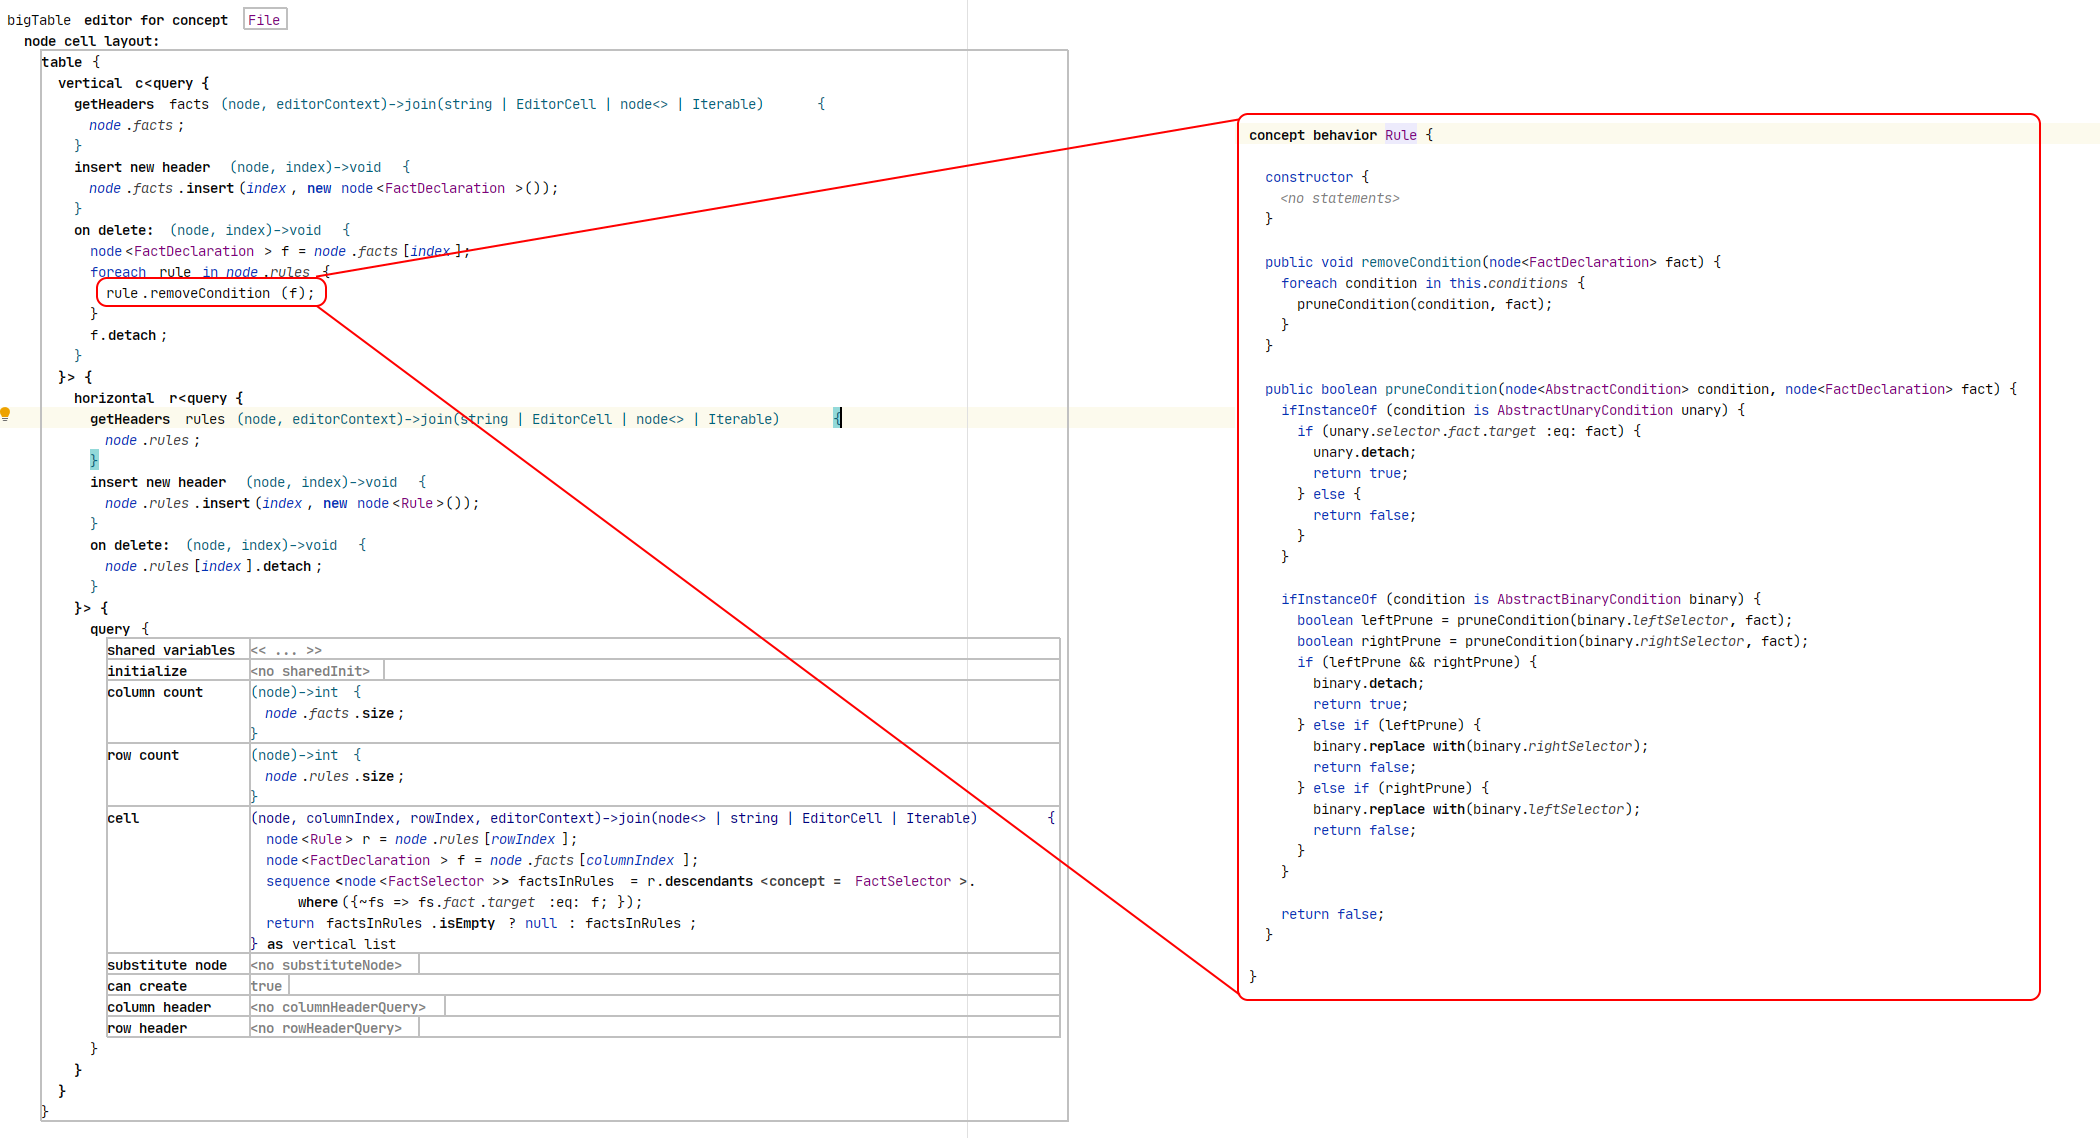
\includegraphics[width=0.99\textwidth]{Sections/images/tableDeleteCode.png}}
    \caption{Table Fact deletion code}
    \label{fig:tableFactDeletion}
\end{sidewaysfigure}

Here we end our experiments in the RSD language.

\newpage

\subsection{Drools-Lite}

Our subsequent experiments were with projections with the Drools-Lite language.
As described in section \ref{section:DroolsLite}, Drools-Lite is an implementation that is much closer to the complete Drools language.
This realism will allow us to create projections that we can present to experienced Drools developers for evaluation.

Of the learnings from the RSD language, one we felt needed fixing to improve understanding was the sparseness of the tables.
By implementing the principle of maximising cohesion, we discovered we could reduce the sparseness issue.
Therefore, as a precursor to our projections, we extended Drools-Lite with a new language that contained one structural item - the \texttt{RuleCollection} Concept.
A \texttt{RuleCollection} node is a child of the \texttt{File} Concept and holds a collection of \texttt{Rule} nodes.
This idea is that related \texttt{Rule} nodes can be placed in the \texttt{RuleCollection}  node to make it easier to examine them together.
This language naturally also added an editor for the \texttt{RuleCollection} Concept.
Additionally, we added intentions to move \texttt{Rule} nodes in and out of groups.

\subsubsection{Decision Table}

As the Drools language is analogous to a series of if-then statements, then perhaps its best visual equivalent is the decision table.
Decision tables are a ``powerful aid in programming, documentation, and in effective man-to-man and man-to-machine communications''\cite{pooch1974translation}.

We designed our table, shown in figure \ref{fig:decisionTableProjection}, to include some of the lessons learned from the RSD crosstab shown in figure \ref{fig:crosstabProjection1}.
The RSD language taught us that wasting visual real estate exacerbates sparseness issues in tables.
In the crosstab table, horizontal scrolling is necessary, in part due to the column widths.
The columns were wide because the name of the \texttt{FactDeclaration} node was displayed horizontally.

\begin{figure}[h]
    \centering
    \fbox{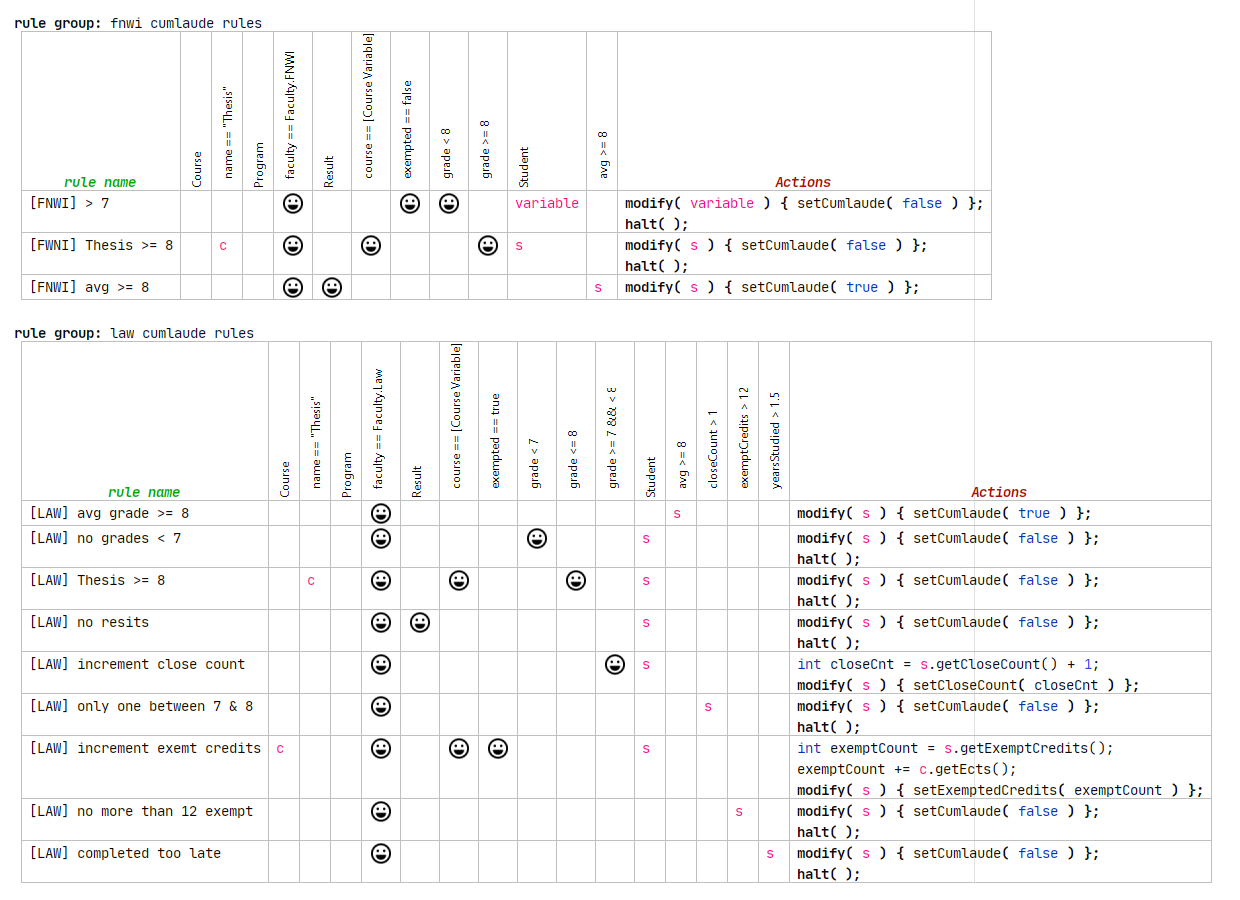
\includegraphics[width=0.99\textwidth]{Sections/images/decisionTableProjection.png}}
    \caption{Decision table projection}
    \label{fig:decisionTableProjection}
\end{figure}

The Drools-Lite language allows for much longer selection criteria on \texttt{FactProperty} references, which would lead to much wider columns.
Our solution was to develop a vertically orientated header cell and use indentation to indicate if the cell is referring to just the \texttt{FactDeclaration} node or a \texttt{FactDeclaration} and \texttt{FactProperty} node combination.

Because this projection presents both the left and right-hand side of the rules, we had to handle the Concept that spans both - the \texttt{RuleVariable} Concept.
We had to find a way to represent a \texttt{RuleVariable} node that can be bound and used on the LHS and used on the RHS.
We achieved this by referencing a \texttt{RuleVariable} node's name in the cell representing the \texttt{FactDeclaration} reference or \texttt{FactProperty} reference to which it is bound.
With \texttt{RuleVariable} nodes now being represented in the cells, we could no longer represent the cell being selected with an ``X'', as this could be confused with a \texttt{RuleVariable} node's name.
Projectional editing does not require communication of meaning through parsable ASCII text.
Thus, we decided to represent \texttt{FactDeclaration} nodes selection with an image.
For arbitrary reasons, we chose a smiley face as that indicator.

The \texttt{Rule} node's names and actions are editable through the default functionality of the MPS extension.
We use intentions to add the selection of a \texttt{FactDeclaration} node or \texttt{FactProperty} reference to a \texttt{Rule} node.
We also use intentions for binding \texttt{RuleVariables}.

The major drawback of this design is that editing a \texttt{Rule} node with yet non-existent selection criteria became very clunky.
If the \texttt{Rule} node we wished to edit already existed in the table, we had to use an intention to extract it from the group, change the criteria and place it back in.
At this point, the table would automatically adjust the column headings.

Experts examined this design in the questionnaire.

\subsubsection{SpreadSheet}

The domain-specific language for the finance world is the spreadsheet.
One study estimated that 90\% of computers had a spreadsheet on them\cite{bradley2009using}.
Dan Bricklin's VisiCalc drove personal computers into the office.
VisiCalc was succeeded by Lotus 1-2-3, which Microsoft Excel then succeeded as the dominant spreadsheet program in the workplace.

This level of familiarity with a paradigm led us to design a projection that had the look and feel of an Excel spreadsheet.
We show this design in figure \ref{fig:SpreadsheetProjection}.
To this end, we created a design where the selection criteria could be directly edited in the cell, as highlighted in the figure.

Each row is a \texttt{Rule} node in this design, and each column is for a \texttt{RuleVariable} node or a \texttt{FactProperty} reference.
If a property is selected, then the selection criterion is in the appropriate cell.
A grey/beige colour indicates unselected cells.
The RHS of the \texttt{Rule} node appears in the Action column.
Adding as yet unused \texttt{FactDeclaration} references or \texttt{FactProperty} references, or removing existing ones, can be achieved with intentions, as shown in figure \ref{fig:SpreadsheetIntentions}, on page \pageref{fig:SpreadsheetIntentions}.

\begin{figure}[h]
    \centering
    \fbox{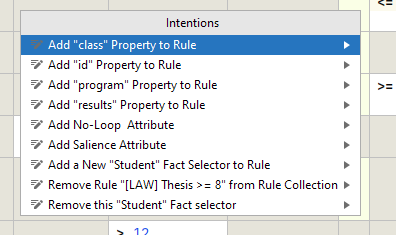
\includegraphics[width=0.55\textwidth]{Sections/images/spreadsheetIntentions.png}}
    \caption{Intention}
    \label{fig:SpreadsheetIntentions}
\end{figure}

This design also allowed us to have more than one selector for the same \texttt{FactProperty} reference, essential for our host organisation's code.
We demonstrate this in figure \ref{fig:TwoProperties}.

\begin{figure}[h]
    \centering
    \fbox{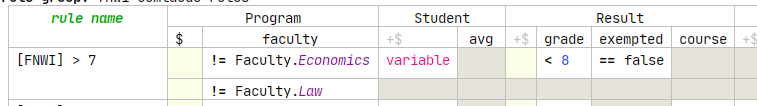
\includegraphics[width=0.90\textwidth]{Sections/images/spreadsheetTwoProperties.png}}
    \caption{Two of same property}
    \label{fig:TwoProperties}
\end{figure}

Experts examined this design in the questionnaire. 
Here we end our experiments in the Drools-Lite language.

\begin{sidewaysfigure}[htbp]
    \centering
    \fbox{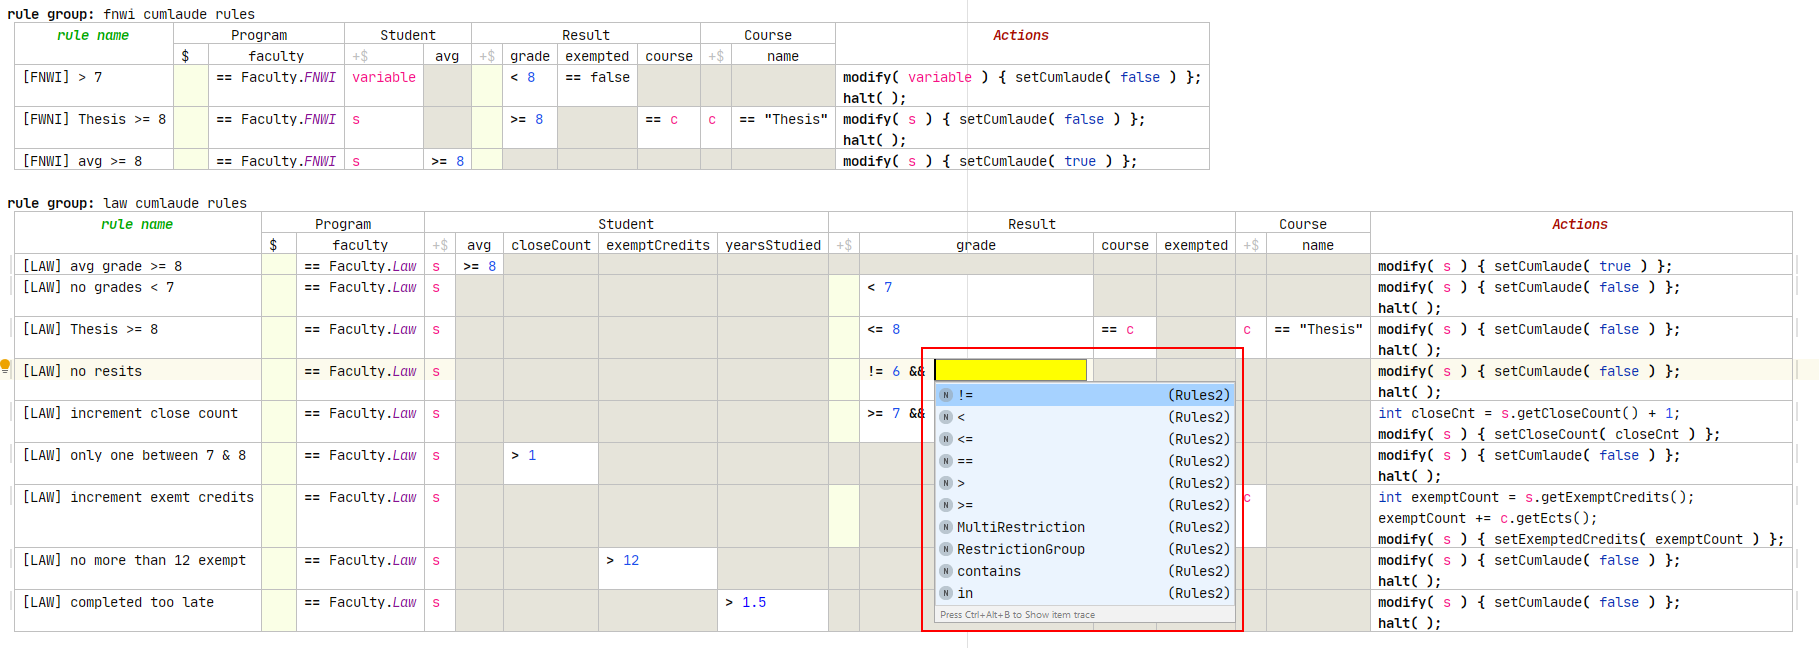
\includegraphics[width=0.99\textwidth]{Sections/images/SpreadsheetProjection.png}}
    \caption{Spreadsheet projection}
    \label{fig:SpreadsheetProjection}
\end{sidewaysfigure}

\newpage

\subsection{Wireframe}

After brainstorming several ideas to present as wireframes to experts as possible projectional aids to understanding, we chose two.
We discuss them briefly in this section.

\subsubsection{Truth Table}
We decided to produce a truth-table wireframe example as we had had personal experience building truth tables to confirm the validity of Drools rules in our work.

The truth table seemed apt for the LHS of the Drools rule as, in essence, it is a boolean function.
Wittgenstein popularised the truth table in the Tractatus Logico-Philosophicus\cite{wittgenstein2013tractatus}.
They are so widely used in mathematics and computer science that we do not need to explain their use further.
Because of the combinatorial explosive nature of truth tables, with 2\textsuperscript{n} possible combinations, we would limit the display to a max of 6 \texttt{FactSelector} nodes and only show the paths that lead to the RHS execution.

Figure \ref{fig:TruthTableProjection} shows how we designed this to look.
The user experience would be that the \texttt{Rule} node is selected, and the developer presses the up and down arrow keys to step through the different true (highlighted in green) and false (highlighted in red) \texttt{FactSelector} nodes that result in the \texttt{Rule} nodes selection.

\begin{figure}[h]
    \centering
    \fbox{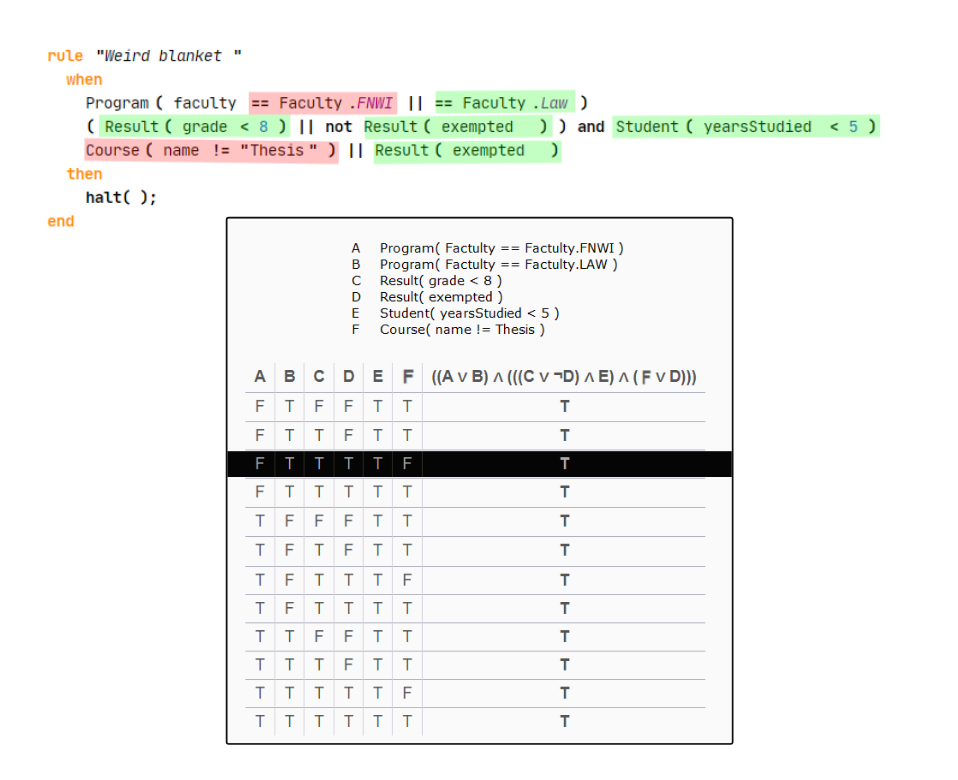
\includegraphics[width=0.80\textwidth]{Sections/images/truthtable.png}}
    \caption{Truth table projection}
    \label{fig:TruthTableProjection}
\end{figure}

We presented this design to our experts to be validated.

\subsubsection{Circuit Diagram}
In our final projection design, we wanted to present a part of projectional editing that we had heretofore only made minimal use of.
That is the use of manipulatable graphics that can change the AST.

We chose a logic circuit. 
The logic circuit represents a boolean operation as NOT, OR, XOR and AND Gates, with their inputs and outputs being inputs to other gates.
In our design, shown in figure \ref{fig:CircuitDiagramProjection}, the input wires to the gates are the \texttt{FactDeclaration} nodes or \texttt{FactProperty} nodes referenced in the LHS.

\begin{figure}[h]
    \centering
    \fbox{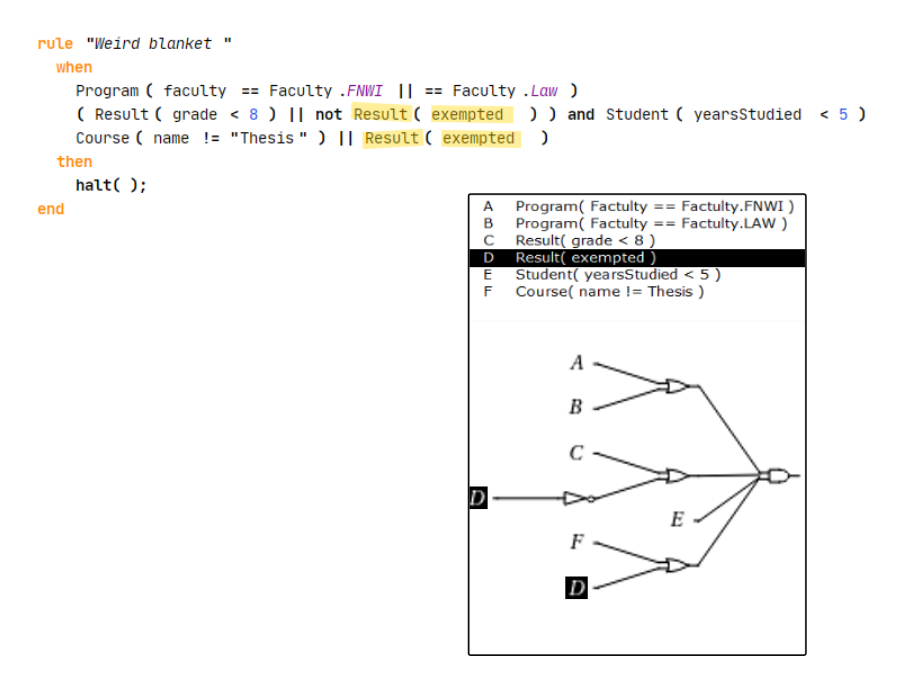
\includegraphics[width=0.80\textwidth]{Sections/images/CircuitDiagram.png}}
    \caption{Circuit diagram projection}
    \label{fig:CircuitDiagramProjection}
\end{figure}

The user experience is that once the \texttt{Rule} node is selected, the developer, by pressing the up and down arrow keys, can step through the different \texttt{FactSelector} nodes (highlighted in yellow) and shown in the circuit diagram, thus showing how the \texttt{FactDeclaration} nodes relate to each other.

We present this design in the questionnaire for validation.

